\chapter{Ablauf}
Im Folgenden wird die theoretische Methodik beschrieben, wie der Einsatz von \gls{KI} zur Optimierung und Steurung der Technik rund um einen Einfamilienhaushalt beitragen kann. Zugrunde liegen drei Phasen, die hierfür durchlaufen werden. Des weiteren sind im Gebäude Voraussetzungen notwendig, die im Folgenden erläutert werden.

\section{Voraussetzungen}
Aufgrund der Vielzahl smarter Gebäudetechnologien (siehe \cref{fig-smart-devices}) und des stark unterschiedlichen Eignungsgrades einzelner Gebäude (in der Spanne vom Althaus mit historischer Bausubstanz bis hin zum Plus-Energiehaus) für ein smartes Upgrade, wird dieser Arbeit ein Modellgebäude zugrunde gelegt. Dies sei ein 4-Personenhaushalt (2 Kinder) in einem freistehenden Einfamilienhaus mit 140 qm Wohnfläche (Entkopplung von Nachbargebäuden, Wohnungen) mit einem Elektrofahrzeug zuzüglich Gas- / Ölzentralheizung neben einer Klimaanlage und elektrischer Rollläden. Internet und WLAN werden vorausgesetzt. Das installieren von steuerbaren Geräten mittels \gls{API} ist nicht Bestandteil dieser Arbeit und wird nicht weiter behandelt. Es wird davon ausgegangen, dass die Daten, auf die zukünftig referenziert werden, programmiertechnisch abgefragt werden können.

\begin{figure}[htbp]
    \centering
    \fbox{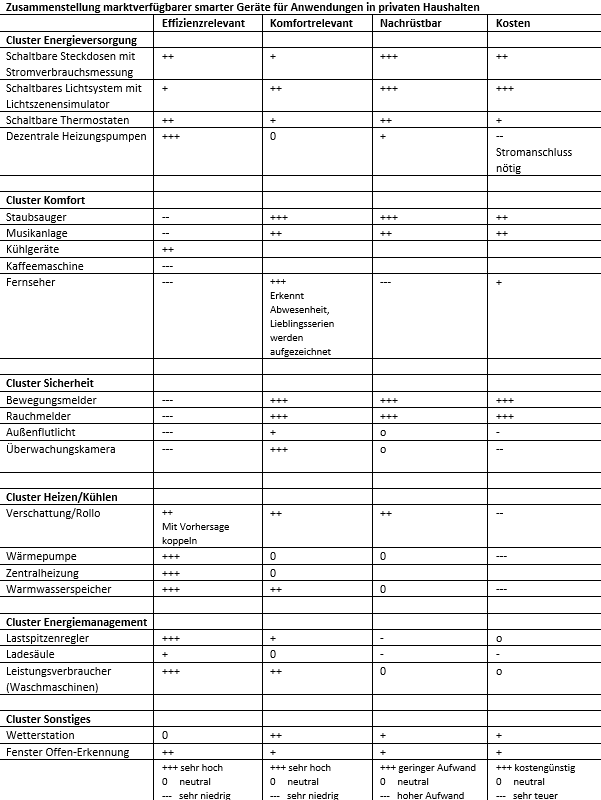
\includegraphics[width=\textwidth]{img/smart_devices.png}}
    \caption{\label{fig-smart-devices}Geräte, die Smart angesteuert werden können inkl. Beurteilung hinsichtlich verschiedener Aspekte}
\end{figure}

\newpage
\section{Neuronale Netze}
Die installierten smarten Geräte liefern also eine Vielzahl von Sensordaten. Diese werden mittels eines tiefen neuronalen Netzes korreliert, um die nutzerkonforme Klassifikation und Betriebsweise der Geräte zu erreichen. In einem abgegrenzten gebäudetechnischen Szenario können dabei Umgebungseinflüsse, wie bspw. Variation der Lichtverhältnisse, Temperatur, Staub etc. auf ein Mindestmaß redziert werden. So ist im Allgemeinen der Einsatz einfacher Techniken, dazu können auch Methoden der Bildverarbeitung aus Überwachungskameras dienen, möglich. Diese Techniken liefern dann eine Objektbeschreibung (sog. Merkmale), wie Kanten, markante Punkte oder Schwellwerte (z.B. sehr helle oder dunkle Punkte in einem Bild), zimmerspezifische Raumtemperatur- und Helligkeitsprofile.

In dem hier zugrundeliegenden Szenario ist jedoch durch die große Variabilität der Umgebungseinflüsse der Einsatz dieser Verfahren nur begrenzt möglich. Deutlich robuster zeigen sich Ansätze, die basierend auf Lerndaten aus wiederholter Prozessbeobachtung  automatisch markante und auf das Szenario angepasste Merkmale zur Objektbeschreibung generieren. Dabei werden Trainingsdaten generiert und einem tiefen Neuronalen Netz zugeführt. Im Gegensatz zu herkömmlichen Neuronalen Netzen bestehen tiefe Netzte aus mehreren verdeckten Schichten (\Cref{fig-deep-nn}). Ein tiefes Neuronales Netz lernt in einem iterativen Prozess komplexe Darstellungen der Eingangsdaten. Die Aussagekraft dieser Darstellungen für das finale Klassifikationsergebnis steigt dabei von Schicht zu Schicht. Basierend auf diesen komplexen Darstellungen (Merkmalen) kann eine zuverlässige Klassifikation und Kategorisierung auch in komplexen Umgebungen abgeleitet werden. Die prinzipielle Vorgehensweise ist in \Cref{fig-deep-nn} dargestellt. Um dies zu erreichen sind folgende Arbeitsschritte erforderlich.

\begin{figure}[htbp]
    \centering
    \fbox{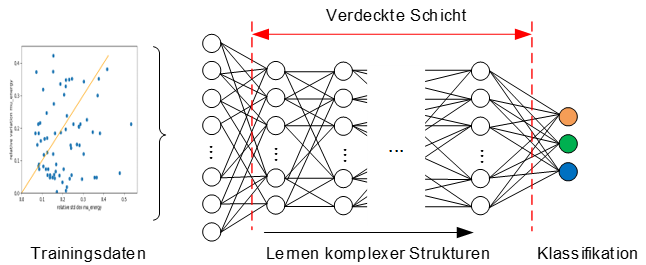
\includegraphics[width=\textwidth]{img/deep-nn.png}}
    \caption{\label{fig-deep-nn}Vorgehensweise zum Lernen komplexer und robuster Merkmalsstrukturen mittels tiefer Neuronaler Netzen}
\end{figure}

\subsection{Generierung von Trainingsdaten}
Um dem tiefen Neuronalen Netz das automatische Generieren von komplexen Merkmalen zu ermöglichen, sind Trainingsdaten notwendig. Dabei müssen in einem Prozess Sensordaten aufgenommen und für das Training relevante Bereiche identifiziert, markiert und ggf. extrahiert werden. Diesen Vorgang bezeichnet man als Labeln, welches von einem Experten durchgeführt wird. Aufgrund der unterschiedlichen Szenarien, Kategorien und der Komplexität des tiefen Neuronalen Netzes ist eine möglichst große Anzahl von Trainingsdaten anzustreben.

\subsection{Lernen komplexer Strukturen mit tiefen Neuronalen Netzen}
Die Struktur des tiefen neuronalen Netzes spielt eine entscheidende Rolle für die Güte der Erkennung. Dazu muss ermittelt werden, was die ideale Konfiguration für die gegebene Problemstellung darstellt (Anzahl der verdeckten Schichten, Anzahl von Neuronen in jeder Schicht, Aktivierungsfunktion, etc.). Die einzelnen Parameter des Netzes werden dabei mittels eines \textit{cross-validation} Ansatzes simuliert und ausgewertet. Um eine stabile und hohe Erkennungsrate im Sinne kurzer Entscheidungszeiten im Prozess zu ermöglichen, wird bei notwendiger Implementierung rechenintensiver Prozesse auf die parallele Verschaltung von Rechner-Hardware zurückgegriffen. Aus Kostengründen im Anwendungsbereich privater Haushalte muss diese Vorlernphase herstellerseitig bewerkstelligt werden.

\subsection{Expertensysteme}
Ein Expertensystem wird als wissensbasiertes System (Knowledge Based System) bezeichnet und stellt einen wichtigen Bereich der Forschung zur \gls{KI} dar. Bei Expertensystemen handelt es sich um intelligente Softwaresysteme, die sich von konventionellen informationstechnischen Systemen in wesentlichen Merkmalen unterscheiden. Der Unterschied zwischen einem wissensbasierten und einem informationstechnischen System lässt sich anhand der Lokalisierung des im jeweiligen System enthaltenen Wissens erklären. Während das Wissen konventioneller Systeme in den Algorithmen und Datenstrukturen durch den Programmierer in der Software implementiert wird, trennt ein wissensbasiertes System strikt zwischen dem „Wissen“ und den Algorithmen zur „Wissensverarbeitung“. Damit wird einem programmiertechnisch nicht versierten Benutzer die Möglichkeit gegeben, die Wissensbasis trotzdem anzupassen. Nach \citefullauthor{Kurbel1992} (\citetitle{Kurbel1992}) ist ein wissensbasiertes System ein Softwaresystem, mit dem das Wissen und die logischen Schlüsse von Experten in einem begrenzten Gebiet nachvollzogen werden. Der praktische Nutzeffekt von Expertensystemen ist dabei die Entlastung der Experten von Routineaufgaben. Typische Charakteristika von Expertensystemen sind dabei die transparente Erklärung der Problemlösung durch Angabe des verwandten Wissens, die flexible Möglichkeit der Erweiterung und Änderung der Wissensbasis und der Entscheidungsstrukturen sowie die hohe Kompetenz in dem bearbeiteten Spezialgebiet. Expertensysteme sind in der Regel für Gebiete entwickelt, auf denen es viele Experten gibt und lassen sich in unterschiedlichen Bereichen einsetzen. So sind sie geeignet für: 
\begin{itemize}
    \itemsep0em
    \item[--] die Interpretation (Interpretationssysteme), d.h. die Auswertung bzw. Analyse von Informationen, z.B. von sensorisch erfassten Daten (Datenanalysen), von akustischen (Sprachverarbeitung), optischen Informationen (Bildverarbeitung) und sonstigen;
    \item[--] die Diagnose von Systemzuständen (Diagnosesysteme), d.h. die Ermittlung von Fehlerzuständen und ihrer Ursachen in Gebäudesystemen (z.B. Fenster offen, Temperatursensor defekt, Licht an/aus);
    \item[--] die konstruktive Gestaltung bestimmter Objekte nach vorgegebenen Spezifikationen (Konstruktionssysteme), z.B. Entwurf (Design) von Sensoren, dezentralen Heizungspumpen mit Hilfe von CAD-Systemen etc;
    \item[--] das Planen von Aktionsfolgen, z.B. beim Einsatz von Leistungsverbrauchern (Waschmaschine, E-Auto laden etc., in der Wärme- und Warmwasserbereitstellung, in der Finanzplanung (Leuchtkörper nach Verbrauchszahlen auswählen und nicht nach Anschaffungspreis, Bestimmung des Return of investment);
    \item[--] das Tutoring (Tutoringssysteme), d.h. Systeme des Lehrens und Lernens (E-Learning-Systeme).
\end{itemize}

Neben dem Einsatz der Expertensysteme in operativen Anwendungsbereichen des Gebäudemanagements, haben diese Systeme eine hohe strategische Bedeutung. Wissensbasierte Systeme dienen dazu, das vorhandene Wissen einer Anwendung systematisch aufzubereiten und zu sichern, zu verteilen und zur richtigen Zeit am richtigen Ort zur Verfügung zu stellen. Die Systeme sind somit wichtige und leistungsfähige Instrumente eines Wissensmanagements.

Kriterien wie Integration, Wartbarkeit, Mensch-Maschine Interaktion (benutzerfreundliche Bedienung sowohl für den Benutzer, als auch für den Experten) und Akzeptanz spielen für den Einsatz von Expertensystemen eine entscheidende Rolle. Mit dem Einsatz eines Expertensystems können sowohl neu entstehende Anforderungen als auch bei der Anwendung auftretende Systemfehler eine Präzisierung der Wissensbasis erfordern.  Es ist somit unabdingbar, dem Benutzer Möglichkeiten zur Wartung des Systems zu bereitzustellen. Die Wartung der Wissensbasis ist zudem häufig erforderlich, da die Aktualität des im Expertensystem gespeicherten Wissens einen hohen Stellenwert besitzt.

Während der Systementwicklung ist der \textit{knowledge engineer} für die korrekte Übertragung des Expertenwissens in das System verantwortlich. Beim Einsatz des Systems hingegen liegt die Verantwortung beim Fachexperten, der als einziger in der Lage ist, die Wissensbasis auf inhaltliche Korrektheit sowie das Expertensystem insgesamt auf ein pragmatisch akzeptables Systemverhalten zu prüfen. Somit erhebt sich die Forderung nach einer für den Experten handhabbaren Schnittstelle für Zugriffe auf die Wissensbasis. Da die Problemlösung durch Expertensysteme auf der Nachbildung des Problemlösungsverhaltens von Fachexperten basiert, stellt die Integration dieser Personengruppe in die Systementwicklung einen wesentlichen Einflussfaktor auf die spätere Benutzerakzeptanz von Expertensystemen dar.

In dem Projekt müssen die charakteristischen Merkmale für die unterschiedlichen Anwendungen identifiziert und später die Auswirkung auf den Gebäudegesamtbetrieb untersucht werden. Ziel ist es durch die Kombination der verschiedenen Sensordaten eine Ist-Zustands-Identifizierung und Charakterisierung zu erreichen.

Das übliche Wirkprinzip der Sensormess-Einrichtungen verlangt eine gewisse \enquote{Vereinzelung} der Messanforderung. Diese Entkopplung verlangt eine Plausibilitätsprüfung der jeweiligen Messwerte, da diese Grundlage für die nachfolgenden Stellgrößen sind. Für den Fall, dass das erforderliche Messprinzip eine aufwändige Datenvereinzelung fordert, ist die Wirtschaftlichkeit der Anwendung zu prüfen. Angestrebtes Ziel ist es die standardmäßige und gefühlte Gebäudeklima-Eigenschaften nicht negativ zu beeinflussen.

Weiterhin wird eine Anforderungsanalyse ermittelt, welche Prozess-, Mess- und Sensordaten zur Optimierung des \gls{TGA}-Betriebs-Prozesses notwendig sind. Auf diese Weise werden unter Berücksichtigung bereits vorhandener Sensorik im Gebäude zusätzlich notwendige Sensorik und ggf. Bilderkennungssysteme (Bewegungsmelder schaltet Kamera ein und setzt z.B. eine Information \enquote{Paket geliefert} oder/und \enquote{Brief zugestellt}, \enquote{Getränke geliefert} ab) identifiziert. Die erfassten Daten werden weiterhin daraufhin untersucht, inwieweit mit ihnen quantifizierbare Aussagen über die Beschaffenheit des Gebäudezustands möglich ist. Dieser Entwicklungsschritt erfolgt in enger Abstimmung mit den Herstellern, Einbau-Fachbetrieben der smarten Geräte und fußt auf Experteninterviews, Prozessanalysen vor Ort und den Ergebnissen einer Anforderungsanalyse. Im Ergebnis wird ein mobiles Sensorsystem mit verschiedenen Sensoren aufgebaut mit welchem alle gebäuderelevanten Daten erfasst werden können. Als Basis für dieses Vorgehen werden verschiede Analyseprogramme und Sensoren genutzt:

\begin{itemize}
    \itemsep0em
    \item[--] OpenCV, Matlab, JMP
    \item[--] Programmiersprachen: Python und C
    \item[--] Verschiedene Temperatursensoren
    \item[--] Verschiedene Helligkeitssensoren
    \item[--] Verschiedene Bewegungssensoren
    \item[--] Verschiedene Zustandssensoren (Heizung, Licht an/aus?, Fenster offen?)
\end{itemize}

Darüber hinaus werden die entstandenen Anforderungen hinsichtlich der Datenkommunikation, -aufbereitung und –speicherung abgeleitet. In besonderem Maße werden die Rahmenbedingungen hinsichtlich der Nutzung der Daten in einem Entscheidungsunterstützungssystem im privaten Umfeld aber auch das zur Verfügung stellen der Daten an die Hersteller zwecks weiterer Optimierung berücksichtigt.

Dies erfolgt in enger Abstimmung mit „Entscheidungsunterstützungssystem“. Auf der Basis der so gewonnenen Erkenntnisse wird eine Systemdefinition für die Datenerfassung erarbeitet. Nach dieser Definition wird sie software- und hardwaretechnisch umgesetzt.

Die Erprobung des Systems zur Identifizierung der unterschiedlichen Anforderungsarten erfolgt in zwei Schritten. Durch isolierte Einzeluntersuchungen der Sensoren werden im ersten Schritt grundlegende Parameter für die Erkennung identifiziert, die später auf verschiedenen Szenarien ohne Rückkopplung in das dortige System evaluiert und ergänzt werden sollen.

Durch die Zusammenführung der unterschiedlichsten Sensordaten soll daraufhin ein Erkennungssystem vorliegen, welches zunächst prototypisch in Bestandsgebäuden installiert wird um einen maximalen technischen Reifegrad zu erreichen. 

Es ist dabei nicht angestrebt alle Sensoren maximal auszuwerten und in einen Entscheidungsprozess einzubinden. Dies ist aufgrund der Komplexität und der Vielzahl der smarten Objekte kaum möglich. Vielmehr wird eine zuverlässige und automatisierte Klassifikation in vorher festgelegte Kategorien angestrebt, die das Ableiten relevanter Parameter für die nachfolgenden Prozessschritte ermöglicht. Dafür sind die Schritte 

\begin{enumerate}
    \itemsep0em
    \item Sensordatenfusion und Generierung von Trainingsdaten
    \item Sensorqualifizierung und Ableitung von Steuerungsparametern
    \begin{enumerate}
        \item Manuelle Merkmalsbeschreibung zur Zustandsidentifikation
        \item Automatische Zustandsanpassung durch Tiefe Neuronale Netze
    \end{enumerate}
\end{enumerate}

erforderlich.

\begin{figure}[htbp]
    \centering
    \fbox{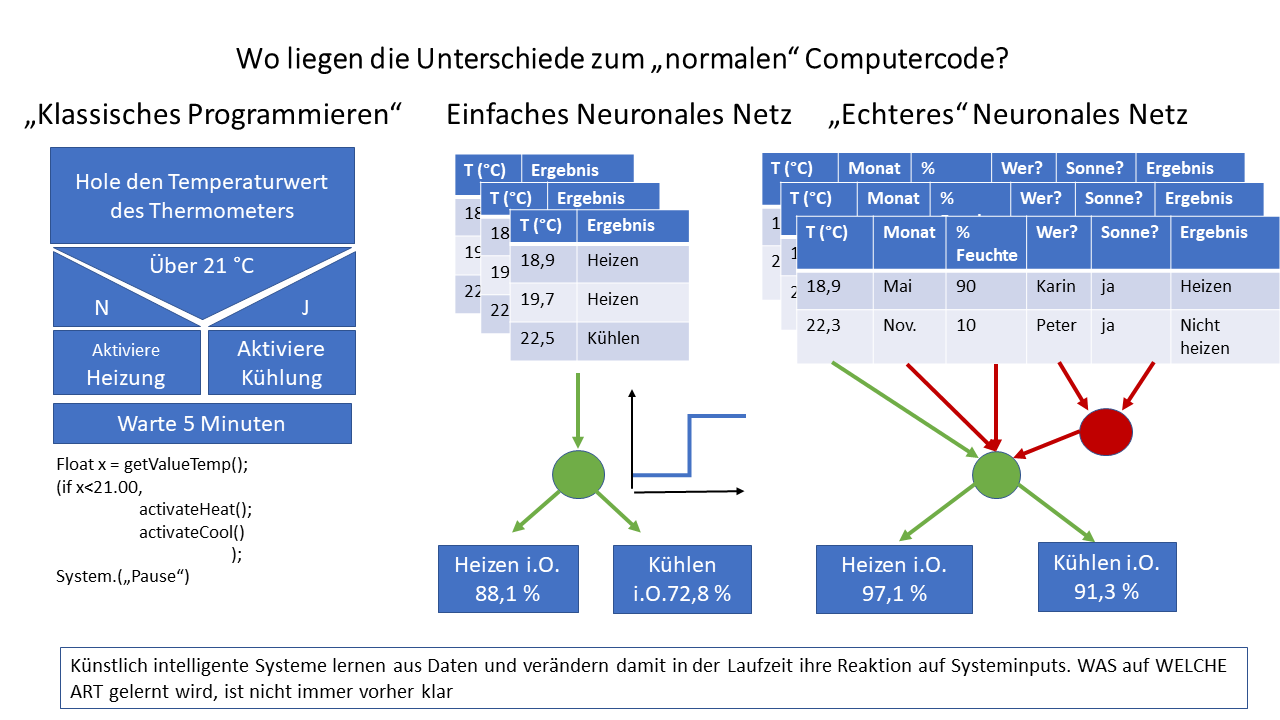
\includegraphics[width=\textwidth]{img/KI Heizen.png}}
    \caption{\label{fig-ki-heizen}Erhöhung der Aussagekraft durch zunehmende Komplexizität der Datenauswertung (von Links nach Rechts)}
\end{figure}

\subsection{Sensordatenfusion und Generierung von Trainingsdaten}
Die Extraktion der Prozessparameter basiert auf einem multimodalen Sensorkonzept. Zu Beginn wird daher die Infrastruktur für die Schnittstellenanbindung der eingesetzten Sensorsysteme an ein Softwareframework aufeinander abgestimmt. Basierend auf diesem Framework können die Daten aus verschiedenen Sensorsystemen z.B. mit korrekten Zeitstempeln versehen und zugeordnet werden (für nachträgliche Auswertung und die Integration von historischen Daten wichtig.

\begin{figure}[htbp]
    \centering
    \fbox{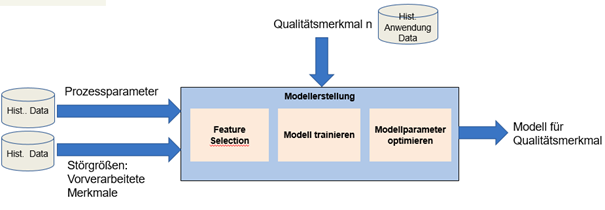
\includegraphics[width=\textwidth]{img/multimodulare Sensorkonzept.png}}
    \caption{\label{fig-multi-kon}Multimodulares Sensorkonzept}
\end{figure}

Das Framework dient als Ausgangsbasis für die Erzeugung von Trainingsdaten. Im Gegensatz zur manuellen Anpassung von Parametern für die Erkennung von Gebäudezuständen werden Verfahren der \gls{KI} eingesetzt. Dabei wird auf eine manuelle Parameteroptimierung verzichtet. Stattdessen müssen Trainingsbeispiele in Form realer Sensordaten bereitgestellt werden, aus denen das System eine optimale Parameterkonstellation automatisch generieren soll.

Die Trainingsdaten werden dabei als Rohdaten / Klassenzugehörigkeit-Kombination verstanden. Dies bedeutet, dass zusätzlich zu den eigentlichen Sensordaten eine Klassenzugehörigkeit angegeben werden muss. Die Klassenzugehörigkeit (z.B.: Kategorie: Lichtszenario) muss durch einen Prozessexperten manuell zugewiesen werden. Die Auswahl der unterschiedlichen Kategorien fließt direkt in die Struktur des finalen Klassifikationsansatzes ein.

Das Erzeugen der Trainingsdaten muss für jeden eingesetzten Sensor separat erfolgen. Durch die Komplexität des Problems und der damit verbundenen Anzahl von Parametern ist eine möglichst große Menge von Trainingsdaten erforderlich. Anzustreben sind dabei 2.000 Rohdaten / Klassenzugehörigkeit Paare.

\subsection{Klassifikation von Gebäudezuständen und Ableitung von Steuerungsparametern}
Dazu werden zwei unterschiedliche Strategien untersucht. Diese sind in \Cref{fig-klassi} dargestellt. Beide Strategien basieren auf Verfahren der KI, wobei Strategie 1 Expertenwissen direkt abbildet und Strategie 2 alle relevanten Prozessparameter aus Beispieldaten direkt am Problem lernt.

\begin{figure}[htbp]
    \centering
    \fbox{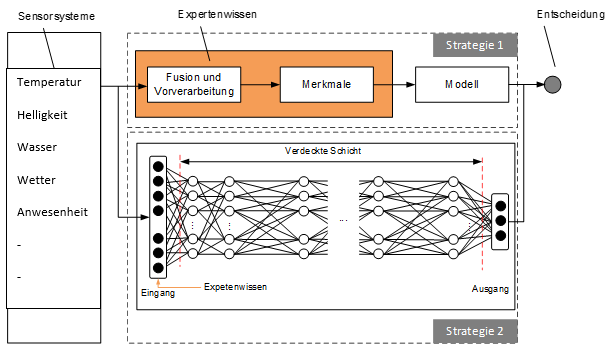
\includegraphics[width=\textwidth]{img/datenklassifikation.png}}
    \caption{\label{fig-klassi}Prinzipielle Struktur eines Verfahrens zur Datenklassifikation }
\end{figure}

\subsubsection{Strategie 1: Manuelle Merkmalsbeschreibung zur Materialidentifikation}
Basierend auf den fusionierten Sensordaten erfolgt die manuelle Ableitung markanter Merkmale. Ziel ist es, durch Kombination und Transformation der Rohdaten aussagekräftige Merkmale zu generieren, die invariant gegen Überbestimmtheit sowie äußere Umgebungseinflüsse, wie bspw. Änderungen der Beleuchtung und Jahreszeiten sind. Hierbei werden gängige Merkmalsbeschreibungen aus verschiedenen Bereichen der Objekterkennung auf das hier betrachtete Szenario portiert. Die extrahierten Merkmale werden in einem Trainingsschritt in ein Modell überführt. Gängige Verfahren sind dabei dem Maschinellen Lernen zugeordnet. Das geeignete Verfahren zur Klassifikation und Modellbildung muss experimentell ermittelt werden. Dieses Modell wird im Weiteren für die Erkennung und Klassifikation des Gebäudezustands eingesetzt. Ziel dieser Strategie ist es, bestehendes Expertenwissen in eine Softwarearchitektur zu überführen, die eine Klassifikationsentscheidung herbeiführt. 

\subsubsection{Strategie 2: Automatische Merkmalserzeugung durch Tiefe Neuronale Netze}
Bei komplexen Problemstellungen mit einer nicht bestimmbaren Anzahl von Umgebungseinflüssen zeigt sich, dass eine manuelle Beschreibung von Merkmalen durch einen Experten oft nicht ausreicht. So werden wirktechnische Zusammenhänge verändert  oder sind unbekannt und können vom Experten nicht abgebildet werden. Robuster ist die automatische und dynamische Auswahl geeigneter Merkmale basierend auf den Gebäudedaten selbst. 

Innerhalb dieser Strategie wird deshalb auf eine manuelle Auswahl von Merkmalen durch Fachleute in eine automatische Merkmalsgenerierung transformiert. Die Merkmale müssen nicht mehr durch die Begutachtung der Analysen durch einen Fachmann identifiziert werden, sondern das neuronale Netz ermittelt die charakteristischen Merkmale über die Trainingsdaten selbst. Nach Abschluss des Trainings sind die Neuronalen Netze in der Lage die Identifizierung des Materials durchzuführen.  

Die Realisierung dieser automatischen Merkmalserzeugung basiert auf tiefen neuronalen Netzen, wie in \Cref{fig-klassi} (Strategie 2) dargestellt. Die Rohdaten werden ohne vorherige Bearbeitung dem Netz zugeführt. Durch die tiefe Architektur und die damit einhergehende große Anzahl von Schichten werden die Rohdaten von Schicht zu Schicht in eine aussagekräftigere Merkmalsbeschreibung transformiert. Das tiefe Neuronale Netz lernt somit automatisch, welche Prozessinformationen entscheidend sind um das vorgegebene Klassifikationsziel (welches in der Rohdaten / Klassenzugehörigkeit Kombination kodiert ist) zu erreichen.

Im Gegensatz zu Strategie 1 benötigt Strategie 2 eine größere Anzahl von Trainingsdaten, da die Parameter gelernt und nicht wie in Strategie 1 von Experten vorgegeben werden. Weiterhin muss die benötigte Struktur des tiefen neuronalen Netzes experimentell evaluiert werden, da eine analytische Bestimmung nicht möglich ist. Beide Verfahren haben im Ergebnis ein Modell zur Klassifikation von Gebäudezuständen sowie eine Bewertung der zugeführten Prozessparameter hinsichtlich Wichtigkeit und Relevanz. Basierend auf diesen Parametern kann im Weiteren ein regelungstechnischer Eingriff erfolgen.

In Abhängigkeit der festgehaltenen Anforderungen in Bezug auf die Identifizierung der Zustände folgt eine Auswahl eines Expertensystems. Gängige Ansätze in der Literatur sind im Wesentlichen:

\begin{itemize}
    \itemsep0em
    \item[--] Simulation
    \item[--] Formale, mathematische Ansätze
    \item[--] Regelbasierte Expertensysteme
    \item[--] Neuronale Netzwerke
    \item[--] Benchmarking
\end{itemize}

Darüber hinaus sind Kombinationen der genannten Ansätze sowie spezifische Ansätze für den Einzelfall denkbar. Alle Ansätze weisen Stärken und Schwächen auf, die hier gegen die spezifischen Anforderungen des Anwendungsfalls abgewogen werden. Eine besondere Herausforderung bei der Auswahl und später bei der Umsetzung eines adäquaten Entscheidungsunterstützungssystems zur Lösung der vorliegenden Problemstellung ist die Einbindung und Verarbeitung der definierten Sensordaten. Je nach Datenvolumen, -komplexität und -geschwindigkeit sind entsprechende Rahmenbedingungen bei der Auswahl und Gestaltung des Systems zu berücksichtigen. Bei der Auswahl des Ansatzes gehen daher Erkenntnisse aus der Datenerfassung ein. Darüber hinaus werden die Schnittstellen der zur Datenerfassung definierten Sensordatenquellen spezifiziert.

Als weiteres wird ein durchgängiges Datenmodell entwickelt, welches Informationen über verschiedene Prozesse hinweg speichert und weitergibt. Die Art dieses Datenmodells hat Einfluss auf die Ergebnisse dieses Arbeitspaketes und muss deshalb berücksichtigt werden. Mit der Nutzung der Informationen aus vorgeschalteten Prozessen, soll der Aufwand der Sensordatenerfassung reduziert und das Ergebnis des Expertensystems verbessert werden.

\begin{figure}[htbp]
    \centering
    \fbox{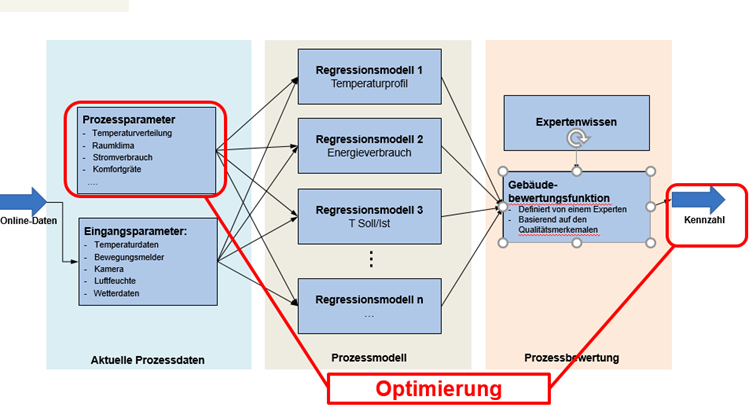
\includegraphics[width=\textwidth]{img/optimierung.png}}
    \caption{\label{fig-opti}Optimierungsprozess zum optimalen Gebäudemanagement}
\end{figure}

Nach der Definition des Entscheidungsunterstützungssystems wird diese softwaretechnisch umgesetzt. Hierzu wird ein agiles, iteratives Vorgehensmodell herangezogen, das über mehrere Prototypen hinweg in enger Zusammenarbeit mit Herstellern der smarten Geräte zu einem einsatzfähigen Entscheidungsunterstützungssystem führt. Ein solches Vorgehen hat den Vorteil, dass Probleme, Fehlentwicklungen und notwendige Anpassungen schnell und effizient erkannt und behoben bzw. umgesetzt werden können. Darüber hinaus kann solch eine Teilevaluierung der angestrebten Problemlösung bereits zu einem frühen Zeitpunkt  durchgeführt werden.

\section{Expertenwissen – Digitaler Zwilling – Hybride Modelle}
Viele Anforderungen an eine effiziente Mess-Steuer-Regeltechnik sind aus dem Bereich der Industrie und des Gewerbes auf Anwendungen der Gebäudetechnik übertragbar. So dienen nicht nur datengetriebene Algorithmen der Optimierung von z.B. Energieverbrauch, auch Expertenwissen und hier insbesondere die individuelle Erfahrung fließt in die Entwicklung von Hard- und Software ein. Dieses Wissen und auch seine Auswirkungen auf den betrachteten Prozess sind jedoch oft nicht quantifizierbar und objektiv zu bewerten. Gleichzeitig werden vielfach Sicherheitsaufschläge in verschiedensten Entscheidungsschritten angewendet, um eine notwendige Qualität zu jeder Zeit gewährleisten zu können. Dies führt häufig zu Ineffizienzen und hohen Energieverbräuchen. Unter Ausschöpfung der Möglichkeiten einer digitalisierten Bewertung von Zuständen sowie intelligenter Datenanalysen und Steuerung der Komponenten der \gls{TGA} können erhebliche Energieeinsparpotentiale realisiert werden, indem die technische Gebäudeausstattung vollautomatisch stets im optimalen Betriebsbereich gefahren werden. Grundvoraussetzung sind hierfür Sensoren, die permanent den Gebäudezustand überwachen, eine Datenakquise, die in der Lage ist, die Informationen dieser Sensoren auszulesen und an geeigneter Stelle zu sammeln, eine kluge Datenaufbereitung, die auch falsche oder fehlende Messwerte sinnvoll verarbeitet, Modelle, die den spezifischen Anwendungsfall richtig beschreiben, und ein digitales System, welches die Situation bewertet, Entscheidungen trifft und umsetzt. Einem solchen System werden Merkmale menschlicher Intelligenz zugesprochen, wenn es die Auswirkungen von Fehlentscheidungen überwacht und künftig vermeidet, also selbsttätig lernt. Die zugrundeliegenden Technologien werden bekanntlich unter den Begriffen Digitalisierung und \gls{KI} zusammengefasst.

Um einen optimalen Betriebszustand herzustellen müssen sämtliche Einflussparameter ins „richtige“ Verhältnis zueinander gesetzt werden um keine Wohnqualitätseinbußen entstehen zu lassen. Die zugrunde liegenden Messwerte sind jedoch natürlichen Schwankungen (z.B. Luftfeuchte, Helligkeitsunterschiede bei Wolkenzug, Windchill-Effekt) unterworfen und somit keinem, rein deterministischen Modell zugänglich.

Die z.T. breite Streuung bei der Zusammensetzung der Messwerte führt somit auch zu deutlichen Schwankungen des Energiebedarfs. Damit ist die gesamte Regelaufgabe sehr stark durch die Erfahrungen einzelner Personen vor Ort beeinflusst. Es ist daher erforderlich, verstärkt den Gesamtzustand zu kontrollieren und die Messwerte zur TGA-Regelung einzusetzen. Die genannten Schwankungen werden häufig mit dem Begriff der „Unschärfe“ (im englischen „Uncertainties“) bezeichnet.

\begin{figure}[htbp]
    \centering
    \fbox{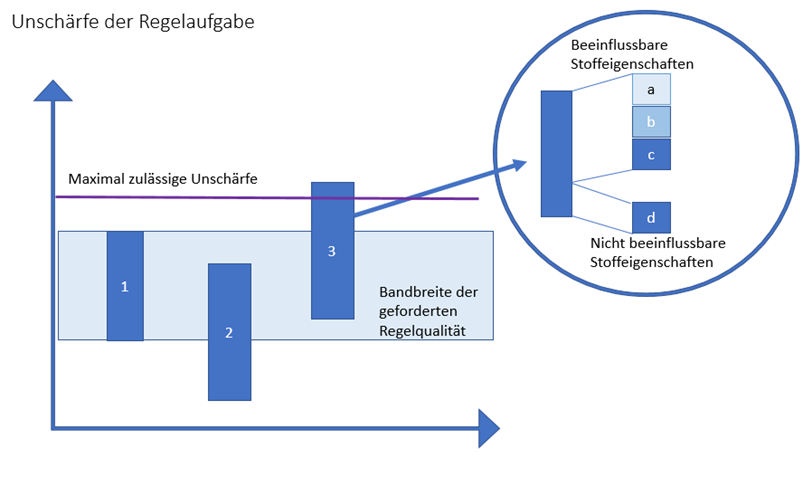
\includegraphics[width=\textwidth]{img/regelaufgabe.png}}
    \caption{\label{fig-regel}Ein Stellbefehl wird aus beeinflussbaren und nicht beeinflussbaren Stoffeigenschaften abgeleitet}
\end{figure}

Die \Cref{fig-regel} zeigt in grafischer Form den generellen Zusammenhang zwischen der Regelqualität und der beschriebenen Unschärfe. Die Balken im Diagramm zeigen auf, dass Schwankungsbreiten der Messwerte hier 1, 2 oder 3 (wie z.B. Luftfeuchte, Gesamtenergieverbrauch oder Strahlungsinternsität (Photovoltaik, solare Wärme)) vorhanden sind. Daher muss in jedem Fall für die Steuerung von diesen Schwankungen ausgegangen werden um trotzdem eine gleichmäßige Regelqualität zu erreichen. Einige der Eigenschaften können bezüglich ihrer Schwankungsbreite beeinflusst werden, andere nicht. Dies zeigt, dass sich eine Optimierungsaufgabe aus einem deterministisch fassbaren Anteil und aus einem nicht mit physikalisch kausal korrelierbaren Anteil zusammensetzt.

So ist der Wärmebedarf eines Heizkörpers abhängig von der Luftfeuchte (Wärmekapazität ändert sich), der Außentemperatur (Fensterflächen und Wände haben unterschiedliche Wärmedurchgangskoeffizienten), dem subjektiven Wohlfühlempfinden (keine physikalische Größe), dem Wolkenbedeckungsgrad etc. Bei vorliegender Soll / Ist-Abweichung ist der Messparameter zur Störgröße geworden.

\begin{figure}[htbp]
    \centering
    \fbox{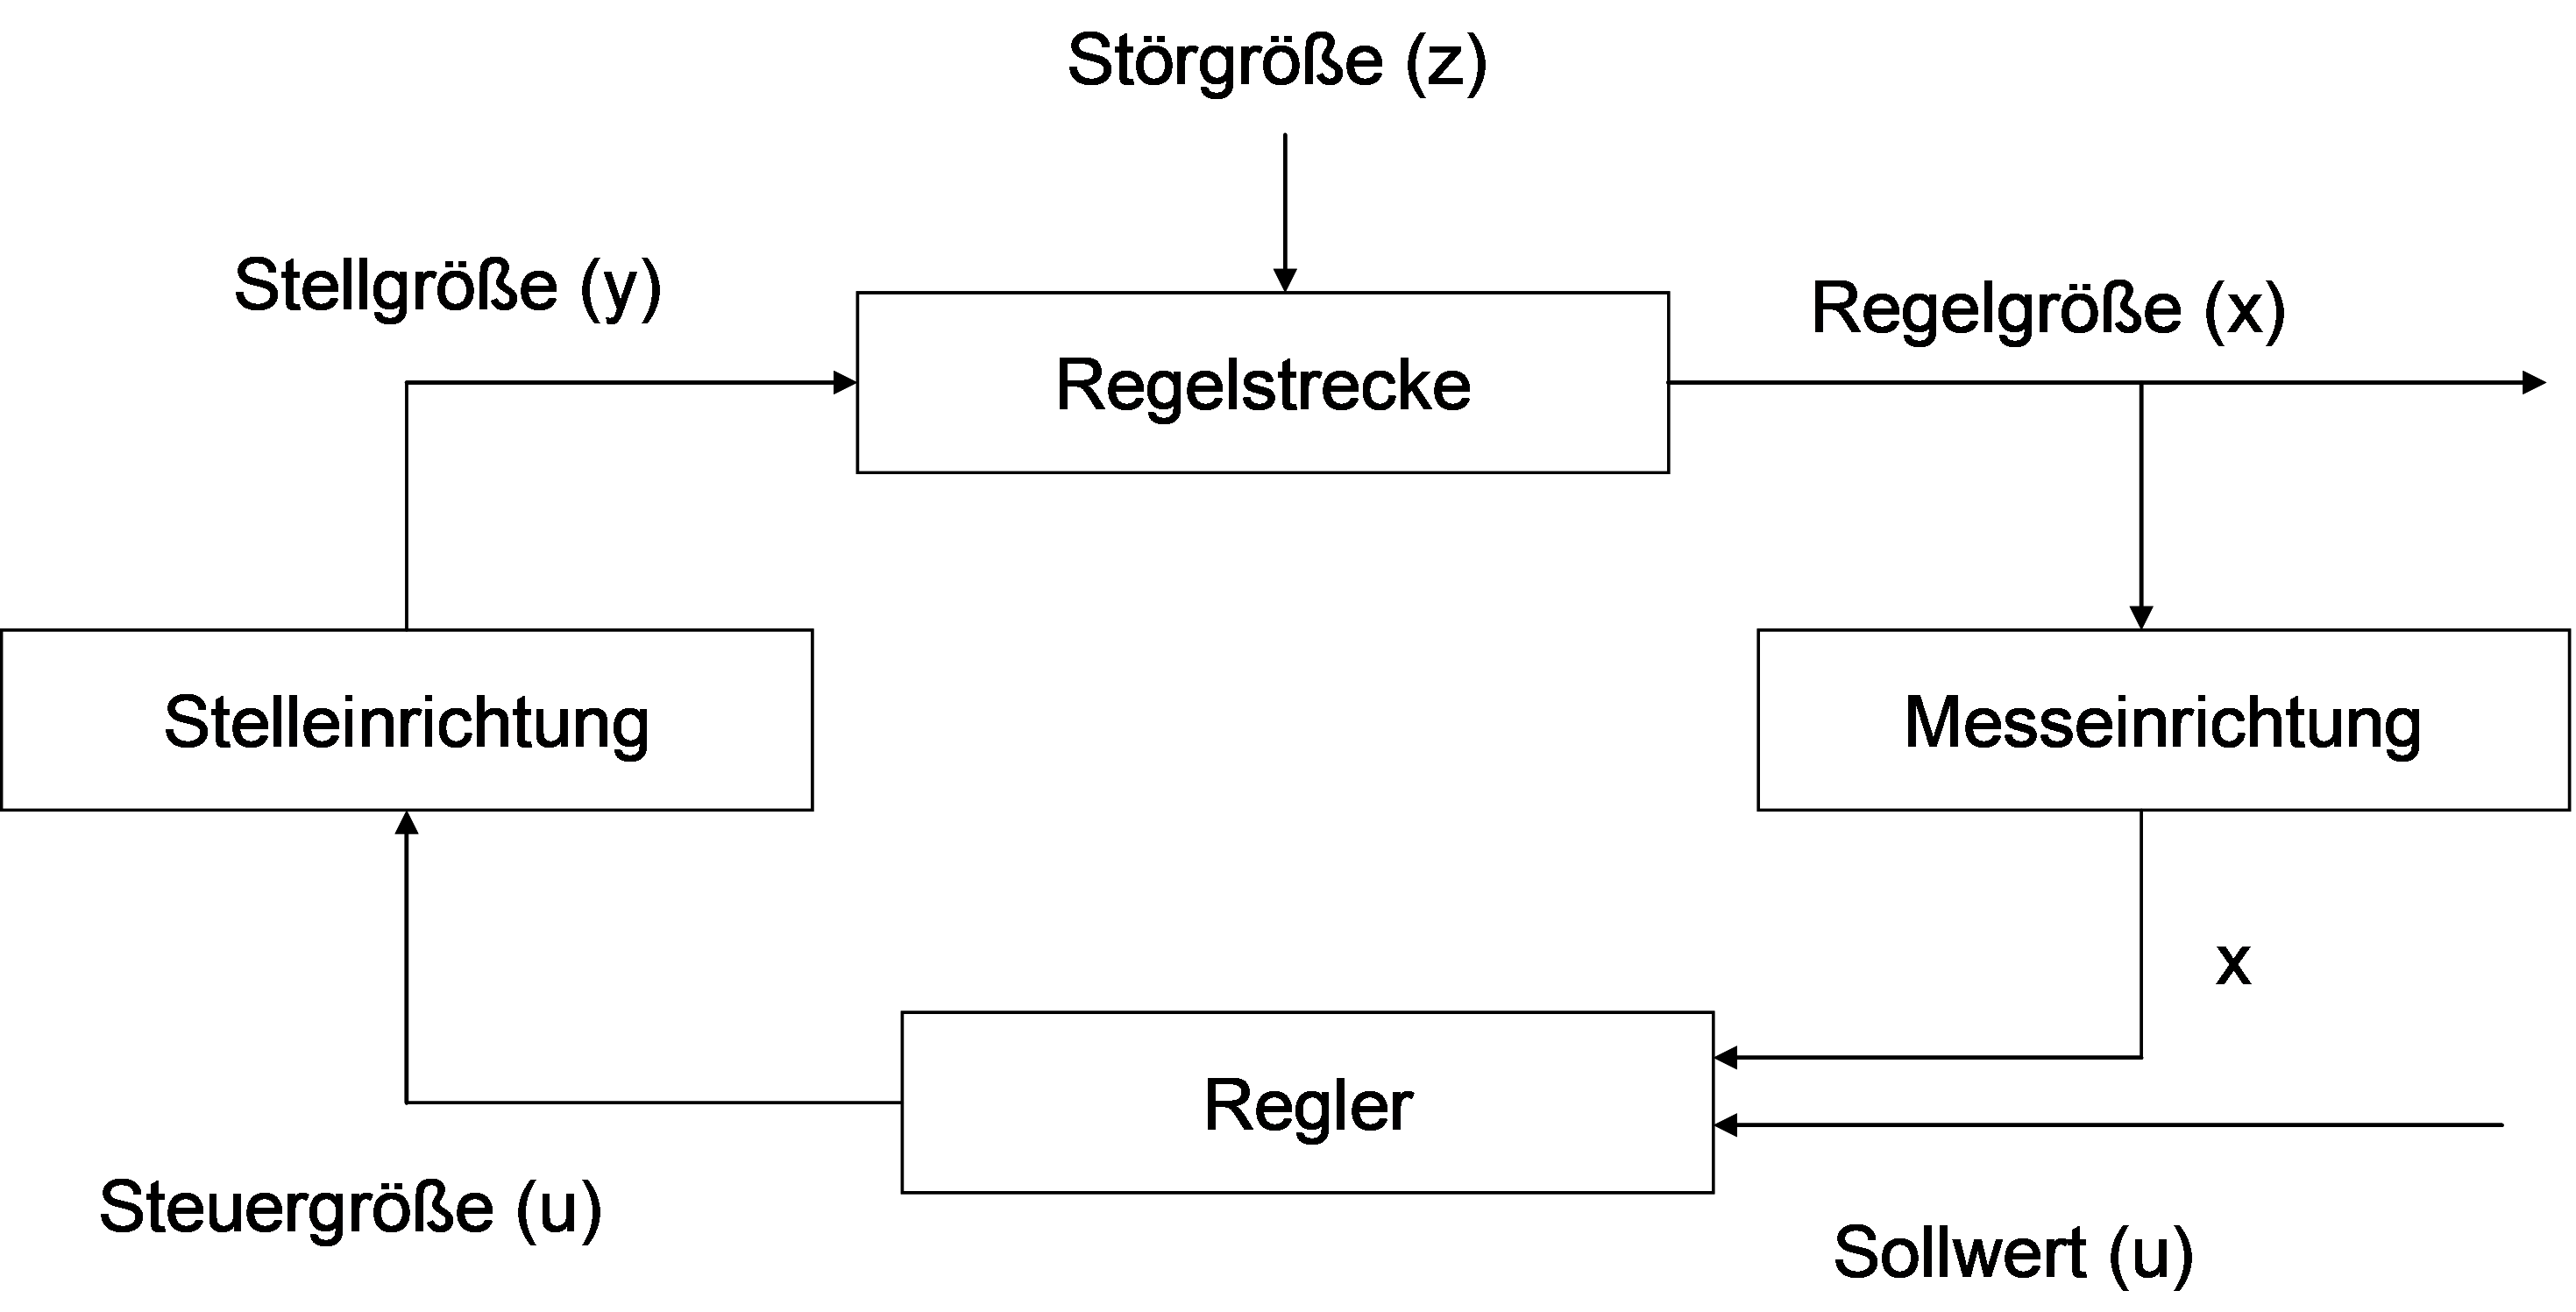
\includegraphics[width=\textwidth]{img/regelkreis.png}}
    \caption{\label{fig-regelkreis}Regelkreis}
\end{figure}

Die Einstellung des idealen Raumklimas lässt sich daher nicht mit einem ansonsten bei vielen Fragestellungen üblichen Regelkreis regeln (ein Beispiel ist in \cref{fig-regelkreis} gezeigt), da nicht nur eine „Stellgröße“ (z.B. die Temperatur) konstant gehalten wird, sondern erhebliche gegenseitige Beeinflussungen aller Parameter (Luftfeuchte, Durchzug, Tür/Fenster auf) auftreten. 

Die Berücksichtigung der beschriebenen „Unschärfen“ soll durch Kombination datengetriebener Neuronaler Netze mit streng physikalischen Gesetzmäßigkeiten erfolgen. Diese physikalischen Gegebenheiten bilden die Grundlage für ein mechanistisches \gls{WBM}. Erweitert man das \gls{WBM} um die digitalisierte Integration der Technischen Gebäudeausstattung, erhält man einen „Digitalen Zwilling“ des Gebäudes und kann rein digital verschiedene Szenarien der Gebäudezustandes vorhersagen. Der Nachteil reiner \glspl{WBM} ist der Umstand, dass nicht alle Phänomene mechanistisch beschreibbar sind und dass Optimierungen aufgrund hoher Rechenzeiten oft nicht echtzeitfähig sind. Dagegen ist der Datenbedarf klein und schnell realisierbar. Das andere Extrem bilden \glspl{BBM} mit nicht immer verfügbaren großen Datenmengen, der Notwendigkeit des maschinellen Lernens und der möglichen Erzeugung von Ersatzmodellen, wodurch eine schnelle und robuste Evaluierung möglich werden kann. 

\begin{figure}[htbp]
    \centering
    \fbox{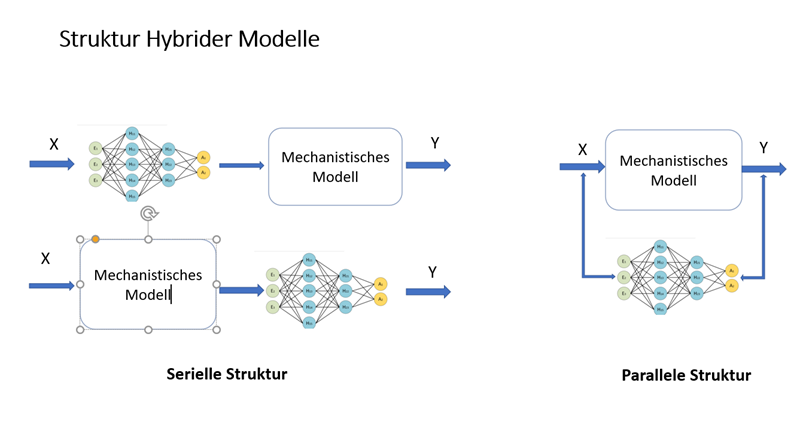
\includegraphics[width=\textwidth]{img/hybrid_model.png}}
    \caption{\label{fig-hybrid}Kombination von \glsfmtshort{WBM} und \glsfmtshort{BBM}}
\end{figure}

Mit der parallelen Struktur lassen sich Fehler der \glspl{WBM} durch \glspl{BBM} „korrigieren“. Die Serielle Struktur hat den Vorteil, Aussagen zu treffen, wenn kein genaues Wissen über die Teilprozesse vorhanden ist, aber genügend Daten vorliegen. 

Beide Modellformen lassen sich nun durch die Kombination der Seriellen Struktur mit der Parallelen Struktur kombinieren, was zu einer deutlichen Reduktion des Datenbedarfs für ein Training führt und Extrapolationen für Bereiche schlechter Datenlage zulässt. 

\begin{figure}[htbp]
    \centering
    \fbox{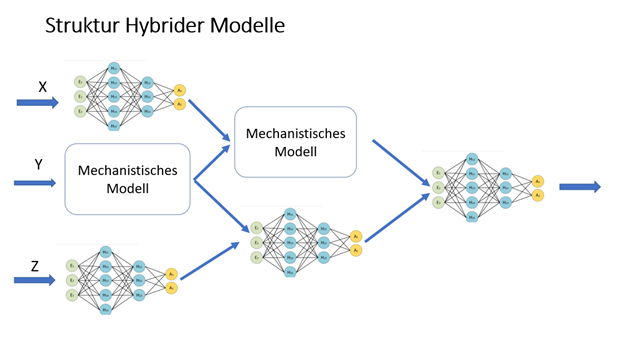
\includegraphics[width=\textwidth]{img/mashed_hybrid.png}}
    \caption{\label{fig-hybrid-mashed}Vereinen der Vorteile paralleler und serieller Hybrider Modelle}
\end{figure}

Da nicht davon ausgegagen werden kann, dass die Hersteller der smarten Geräte ein einheitliches Datenformat verwenden und sich einer standartisierten Datenschnittstelle bedienen, erscheint die Anwendung des Hybriden Kombinationsmodelles gemäß \Cref{fig-hybrid-mashed} der zielführende Lösungsansatz zu sein. Ferner sind Plausibilitätstests sowohl von Sensorrohdaten als auch von Vorhersage-Soll-Größen durch Abgleich mit gebäudetechnischen Modellen möglich.

\section{Datenintegration}
Um die Daten aus der Vielzahl verschiedener Smart Home Geräte (siehe \cref{fig-smart-devices}) auszulesen und weiterzuverwenden, wird ein passendes System benötigt. Dabei gilt es folgende Voraussetzungen zu beachten: Das System muss

\begin{itemize}
    \itemsep0em
    \item[--] Daten unterschiedlicher Formate einheitlich ablegen,
    \item[--] Eigenständig, in bestimmten Intervallen, Daten der einzelnen Geräte anfragen,
    \item[--] Daten durch eine REST-Schnittstelle abrufbar machen,
    \item[--] Daten für eine Langzeitspeicherung optimiert ablegen und
    \item[--] Zukunftssicher Daten im Big Data Bereich verarbeiten können.
\end{itemize}

Diese Anforderungen werden von der Plattform \textit{Splunk} erfüllt.

\begin{figure}[htbp]
    \centering
    \fbox{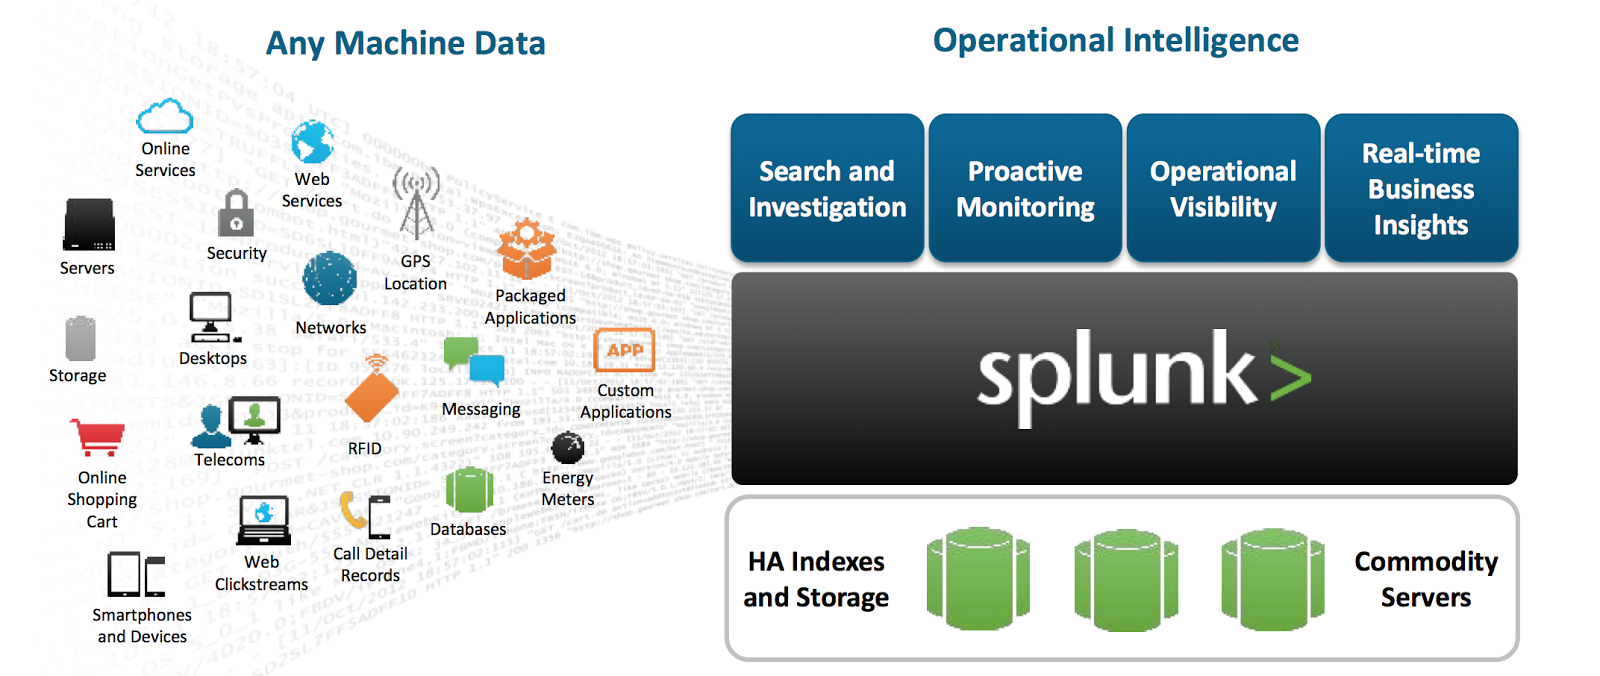
\includegraphics[width=\textwidth]{img/splunk_umfang.png}}
    \caption{\label{fig-splunk} Die unterschiedlichen Datenquellen und Anwendungsarten der Splunk Plattform}
\end{figure}

\paragraph{Splunk} ist \enquote{eine skalierbare und zuverlässige Datenplattform zur Untersuchung, Überwachung, Analyse und Bearbeitung von Daten}. \cite{splunk2021} Die Plattform setzt dabei auf das Motto \enquote{One Platform to Rule Them All}, also dass eine Plattform alles können soll. Die Stärke von Splunk ist, dass es aus nahezu jeder Quelle Daten lesen, umstrukturieren und ordnen kann. Dabei arbeitet Splunk standardmäßig mit Zeitstempeln und labelt jeden gelesenen Datensatz mit einem entsprechenden Stempel. Die Struktur der Daten liegt dabei komplett in der Hand des Administrators der Plattform, da Splunk diesbezüglich keine Voraussetzungen hat.

\Cref{fig-splunk} ist zu entnehmen, dass Splunk Daten aus einer Vielzahl an Quellen aufnehmen, verarbeiten und visualisieren kann. Die Auswertungsfunktionen für Daten lassen es auch zu, dass eine \gls{KI} inklusive maschineller Lernalgorithmen in der Plattform selbst verwendet wird. Diese Art von Datenspeicher ist sehr modular, da neue Geräte einfach mit einer eigenen Spezifikation hinzugefügt werden können. Ein Grundbedürfnis an funktionalität auf der Geräteseite wird aber dennoch Vorausgesetzt, dies ist aber unumgänglich.

Splunk kann sowohl die Daten für eine dritte Anwendung zur Weiterverarbeitung über mehrere Schnittstellen bereitstellen, als auch als eine eigene Oberfläche zur Kontrolle und Steuerung der \gls{TGA} fungieren.